\documentclass[a4paper]{jpconf}
\usepackage{graphicx}
\begin{document}
\title{PyFAI, a versatile library for azimuthal regrouping}

\author{J\'er\^ome Kieffer, Dimitris Karkoulis}

\address{European Synchrotron Radiation Facility; 6 rue Jules Horowitz;
38043 Grenoble; France}

\ead{jerome.kieffer@esrf.fr}

\begin{abstract}
Area ($2d$-) detector like CCD or pixel detectors have replaced punctual detector
over the 15 last years in diffraction (both in WAXS, SAXS and single crystal
diffraction). Those detectors with wide sensitive area have micron-sized spatial
resolution and provide millions of pixels. PyFAI was designed to reduce SAXS and
WAXS images taken with those detectors into $1d$ curve (azimuthal integration)
or $2d$ images (transformation named caking), usable by other software like Rietveld
refinement tools.

As a library, the aim of pyFAI is to be integrated in other tools like PyMca[]
or EDNA\cite{edna} with a clear pythonic interface. But pyFAI offers also
command line tools for batch processing, exporting data in q-space (for SAXS) or 2$\theta$ for
(WAXS) and a calibration GUI for optimizing the geometry of the setup starting
from  reference sample's “powder rings”.  PyFAI shares the geometry of
SPD\cite{spd} but can directly import geometries determined by
Fit2D\cite{fit2d}.
PyFAI has been designed to work with any kind of detector and geometry (transmission or reflection) and
relies on fabio; a library able to read more than 20 image formats
produces by  detectors from 12 different manufacturers.

Even if the basic idea is interpolation from cartesian space $(x,y)$ to polar
space $(2\theta, \chi )$, intensities should be conserved (both local and total)
to get quantitative results.  Those technical details on how integration is implemented
and how it was ported to native C-code and parallelized on graphic card are
discussed  in this paper.
\end{abstract}

\section{Introduction}

With the advent of hyperspectral experiments like diffraction tomography in the
world of synchrotron radiation, existing tools for azimuthal integration like
Fit2D\cite{fit2d} and SPD\cite{spd} reached their limits with the fast data rate
needed by such experiments. Even when integrated into massively parallel
frameworks like EDNA\cite{edna}, such stand-alone programs, due to their
monolithic nature,  could not keep pace with the data flow of new detectors.


\section{Fast azimuthal integration}
This highlights the need for a new tool performing azimuthal integration much
faster than before, without compromising quality. Python is a very popular
platform for data analysis tools (PyMCA\cite{pymca}, PyNX\cite{pynx}, \ldots)
which is appreciated by scientists and already widely used in the community.
This tools should also be open-source to allow control of the results and
further adaptation to specific needs.

\subsection{PyFAI executables}
PyFAI was designed to be used by scientists needing a simple tool for azimuthal
integration. Two command line programs “pyFAI-waxs” and “pyFAI-saxs”
which are provided with pyFAI for performing the integration of one or many
images.The WAXS version outputs results in $2\theta /I$  whereas the SAXS version outputs $q/I(/\sigma )$.
Options for those programs are parameter  files describing the geometry and mask file. They can
also do some  pre-processing like dark-noise subtraction and flat-field correction.


\subsection{A Python library}
But pyFAI is first and foremost a library, another tool add to the scientific
toolbox built around ipython\cite{ipython} and numpy\cite{numpy} allowing the
design of data analysis scripts to be written in minutes: defining an ``integrator'' object is done in a
single line and integration of an image is done in a single call to the library.

\begin{center}
\begin{figure}[h]
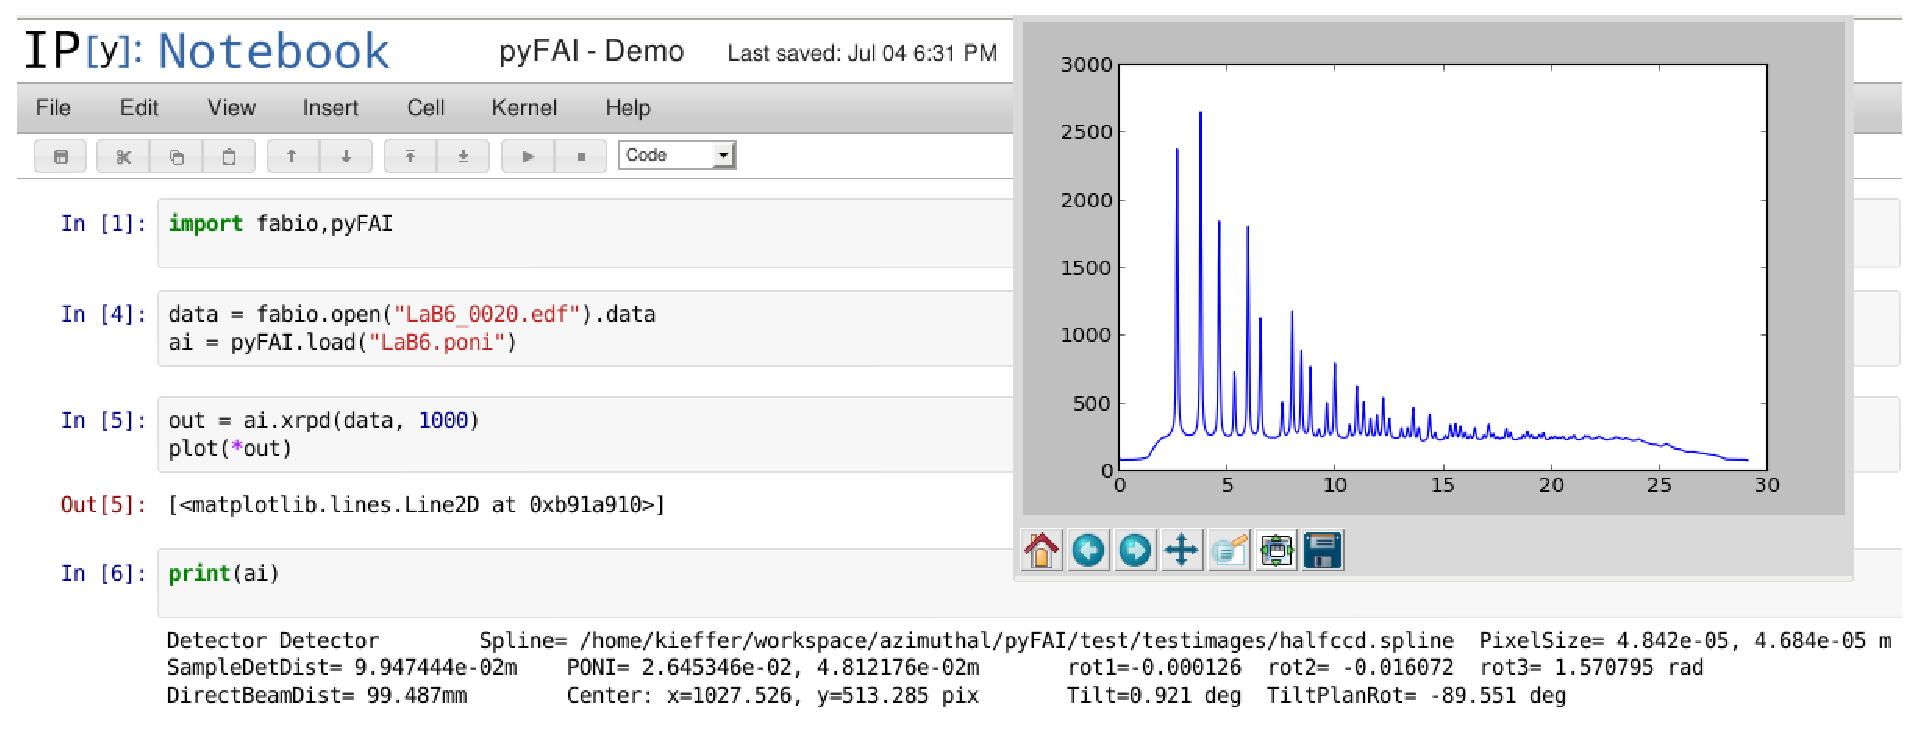
\includegraphics[width=15cm]{img/notebook-l.eps}
\caption{\label{notebook} Example of interactive use of fabio and pyFAI in the
interactive environment ipython (here the notebook interface).}
\end{figure}
\end{center}


\section{Regrouping mechanism}
Azimuthal-regrouping is done in pyFAI using a histogram-like algorithm: every
pixel of the input image is associated to it's coordinate in polar coordinate
$(2\theta , \chi )$ or $(q, \chi )$. Then a couple of histograms of $2\theta$
(or $q$) are build:
one non weighted for measuring the number of pixels falling in each bin and
another weighted by pixel intensities.
The division of the weighted histogram by the number of  pixels per bin gives
the powder pattern.
$2d$ regrouping (called caking in FIT2D) is obtained in the same way using
two-dimensional histograms over radial ($2\theta$ or $q$) and azimuthal angles
($\chi$).

\subsection{Pixel splitting algorithm}
Powder diffraction patterns obtained by histogram have a major weakness where
statistic is low: a high level of  noise is observed close to the beam
stop.
This is particularly striking when considering  $2d$-regrouped where most of
the bins close to the beam-stop are not populated by any pixel. As we can
see on Figure \ref{rough} most of the area affected by this is shaded by the beam-stop, but such a compromise was not acceptable:
the  $2d$-regrouping of a smooth image should be smooth (Figure \ref{smooth}.

\begin{center}
\begin{figure}[h]
\begin{minipage}{8cm}
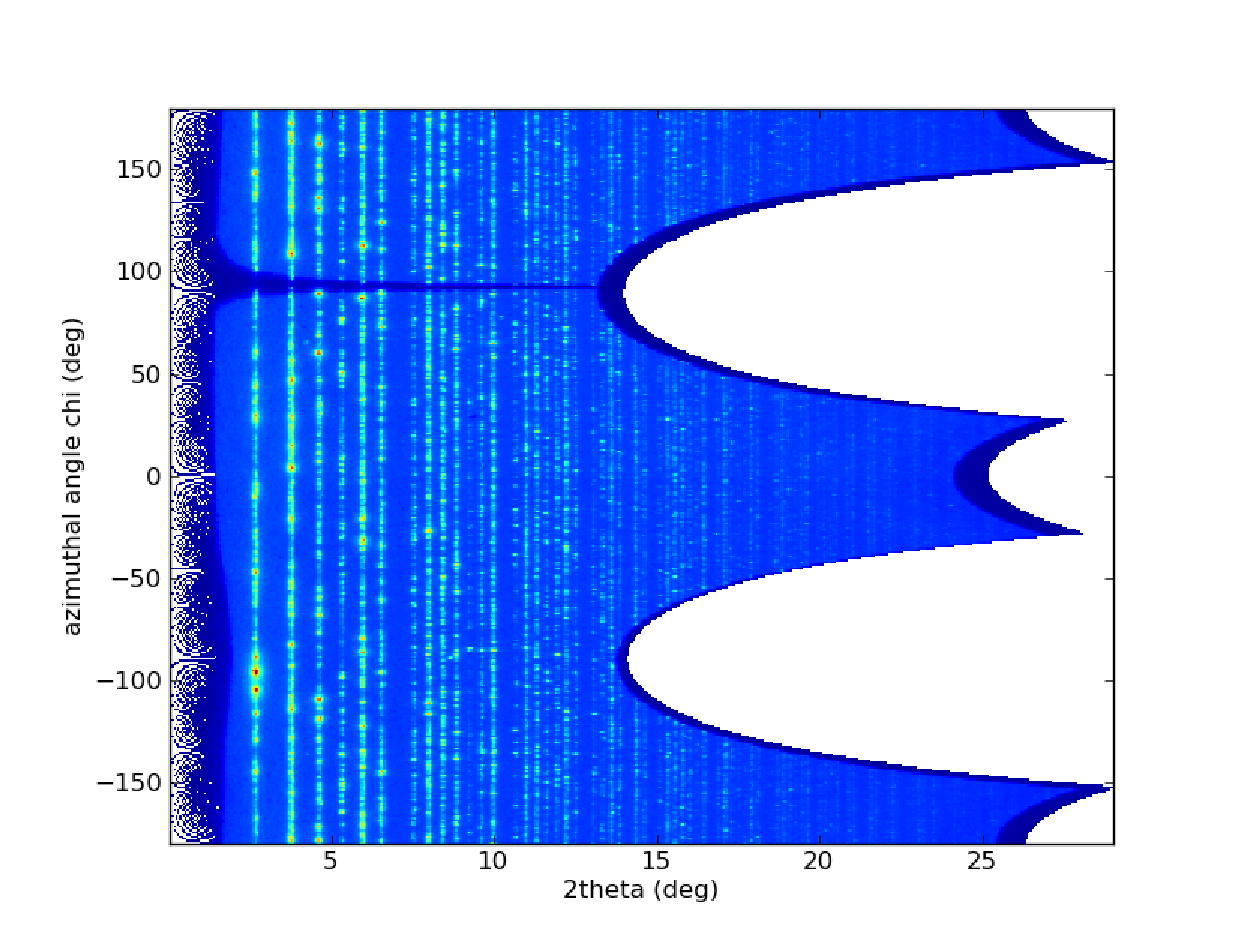
\includegraphics[width=8cm]{img/2Dhistogram.eps}
\caption{\label{rough}$2d$-regrouped image without pixel splitting. Note the
missing pixels near the beam stop and the high-frequency noise patterns.}
\end{minipage}\hspace{5mm}
\begin{minipage}{8cm}
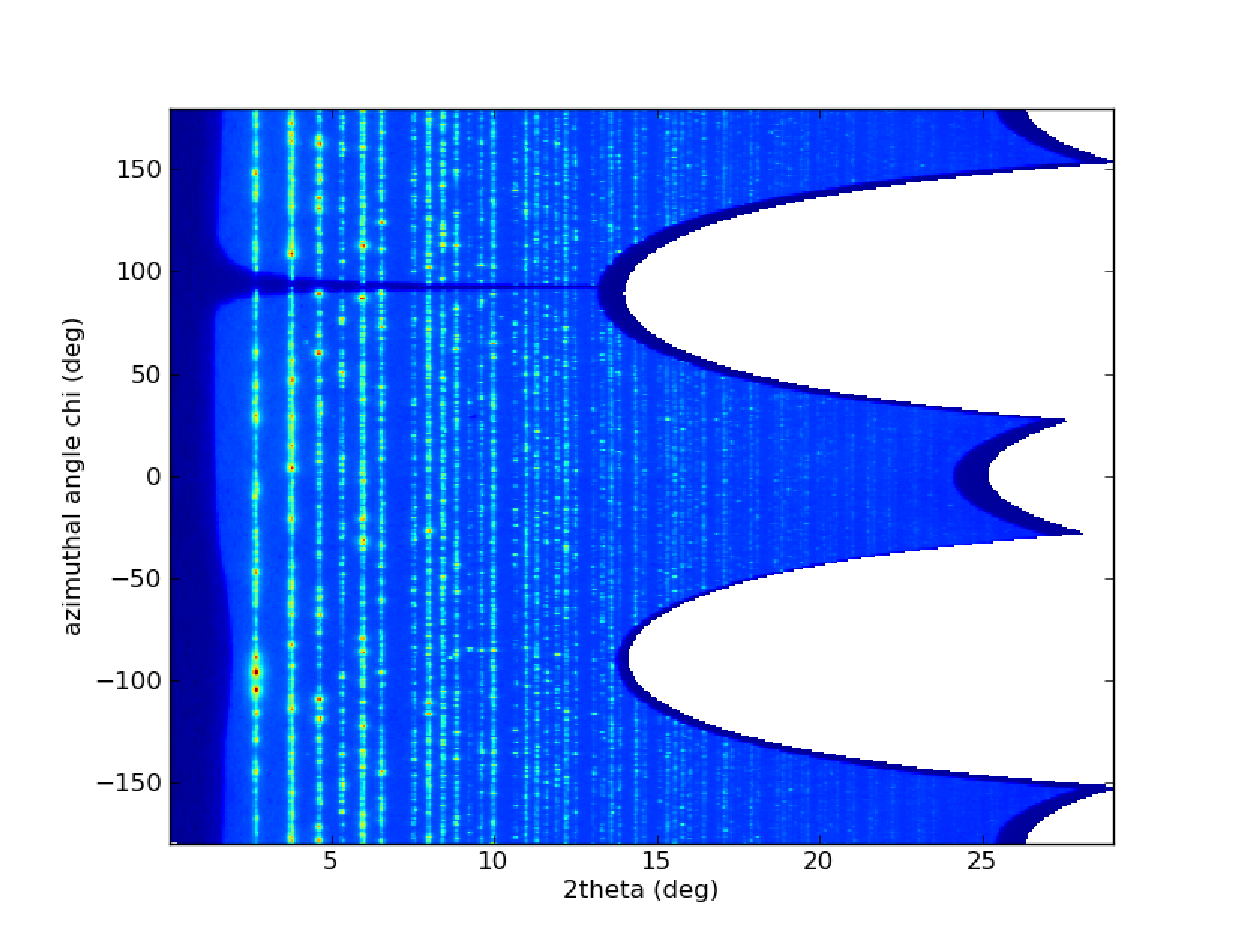
\includegraphics[width=8cm]{img/2DwithSplit.eps}
\caption{\label{smooth}$2d$-regrouped image with pixel splitting. The
transformation of a smooth image remains smooth.}
\end{minipage}
\end{figure}
\end{center}

PyFAI solves this problem by considering in addition to the position, the
spatial extension of every pixel. Every pixel is then splitted and distributed
over the corresponding bins; intensity being homogeneous over a
single pixel.

\subsection{Performances and migration to native code}
Computation time is proportional to the size of the input image and almost
independent of the number of bins. Originally the regrouping was implemented
using the histogram and histogram2d provided by numpy\cite{numpy}. As this step
is the most  time consuming, it was re-implemented and optimized using
cython\cite{cython} to achieve  a  four times speed-up.
The pixel splitting algorithm was also implemented in cython, enhancing the
original histogram and optimized to give excellent single-threaded performances
around 30 Hz.Mpixel.

\subsection{Graphic card implementation}
Graphical Processing Unit (GPU) are composed of hundreds of
small computing cores; they are optimized for highly parallel algorithms
with speed-ups going up to 3 orders of magnitude over sequential code running
on Central Processing Unit (CPU).
While histograms do not fall into this category, they can  nevertheless be
ported to GPU efficiently. In order to benefit from GPU acceleration, the Open
Computing Language (OpenCL) was used. OpenCL can make use of multiple  different
devices such as CPUs and GPUs with very different features and capabilities.
This framework also allows the code to work on multiple CPU cores, which was
useful for validation. Azimuthal integration is a reduction
of millions of pixels to hundreeds of bins, so processing needs to be done in
double-precision; which is not available in all devices. Table{perfs} sumarizes
the execution time

\subsection{Performances}
\begin{table}[h]
\caption{\label{perfs}Performances obtained on a computer with two Intel
XeonX5690 @3.47GHz and various GPU: C2075 and GTX580 are professional and consumer grade Fermi class nVidia GPU with 512 cores.\\
 The table reports execution time measured in milliseconds on various size of
 images in double precision except for the AMD FireGL v7800 where single
 precision had to be used).}
\begin{center}
\begin{tabular}{|l|c||c|c||c|c|c|c|}
\hline
Image               & Image size 	& \multicolumn{2}{|c||}{CPU X5690}& \multicolumn{4}{|c|}{OpenCL $1d$ regrouping} \\
					& mega pixels	& $1d$	&	$2d$	&	X5690	&	C2075	&	GTX580	&	FireGL* \\
\hline
Pilatus-1M 			& 1  			& 34.4  &	63.1	&	13.9	&	7.2		&	6.3		&	13.8 \\
Half-Frelon 		& 2  			& 76.6  &   132.4   &	23.4	&	14.4	&	12.2	&	18.8 \\
Frelon 				& 4  			& 165.0	&	269.4   &	52.6	&	34.1	&	28.2	&	40.0 \\
Pilatus-6M 			& 6  			& 232.0	&	350.7	&	74.4	&	49.8	&	40.7	&	48.1 \\
Fairchaild 			& 16 			& 613.9	&	849.7   &	158.9	&	99.0	&	96.4	&	95.6 \\
\hline
\end{tabular}
\end{center}
\end{table}

The OpenCL implementation of pyFAI is very fast on GPU offering an extra five
time speed-up over CPU implementation. The profiling of the code revealed new
bottlenecks which will be addressed in futur optimisations.

\section{Conclusion}


A library such as pyFAI has two main goals:
\begin{itemize}
\item Performing azimuthal integration witch offers a clean interface to
developers or scientists in the field of X-ray diffraction and provide outstanding performances.
\item No compromise on the quality of the result with a carreful management of
the geometry and precise pixel splitting offerting total and local intensity
conservation.
\end{itemize}

This twenty folds speed up in azimuthal integration opens the door to a new
kind of analysis, not even considered until today: a scientist could write
himself a small script of a dozen of lines of code for analyzing a diffraction
tomography experiment (typically 60 x 200 frames), such analysis would only
take a few minutes using pyFAI when it used to take days for data reduction only.
PyFAI is the tool to couple with the next generation hi-speed detectors.

\subsection*{Acknowledgments}
Authors wishing to acknowledge assistance from
colleagues, especially Manuel S\'anchez del R\'io for suggesting the usage of
of weighted histograms;
V. Armando Sol\'e for his expertise on developing native code under windows,
Jonathan Wright and all the ESRF-ID11 team for the specification and Peter B\"osecke for
the geometry used in pyFAI. Porting pyFAI to GPU would not have been
possible without the financial support of LinkSCEEM-2 (RI-261600).

\subsection*{Appendices}
PyFAI is an open source software released une the GPL licence.
As of July 2012, pyFAI is available in version 0.6 on the EPN-Campus forge
(https://forge.epn-campus.eu/projects/azimuthal) which includes OpenCL
acceleration.
PyFAI depends on Python v2.6 or v2.7, numpy\cite{numpy} and OpenCL\cite{opencl}
In order to be able to read images from various detector, pyFAI relies on the
fabio library available from sourceforge. The graphical user interface for
calibration of diffraction setup uses in adition matplotlib\cite{matplotlib},
scipy\cite{scipy}, and FFTw3\cite{fftw}.
C, C++ and Cython compilers are needed to build pyFAI from source.

PyFAI is packaged and available in common Linux distributions like Debian
7.0 and Ubuntu 12.04. Install packages for Windows are also
available on the EPN-Campus forge.

 \section*{References}
\bibliographystyle{iopart-num}
\bibliography{biblio}

\end{document}


